\documentclass[12pt, a4paper]{article}

% --- PACKAGES ---
\usepackage[utf8]{inputenc}         % Crucial for UTF-8 character support
\usepackage[margin=2.5cm]{geometry} % Set page margins
\usepackage{booktabs}               % For professional-looking table lines
\usepackage{caption}                % For better control over captions
\usepackage{amsmath}                % For advanced math environments
\usepackage{graphicx}               % To include graphics
\usepackage{hyperref}               % For clickable links and references
\usepackage{tikz}                   % For drawing
\usetikzlibrary{positioning}
\usetikzlibrary{positioning}
\usepackage{pgfplots}               % For creating plots and charts
\pgfplotsset{compat=1.17}            % Use a recent version of pgfplots
\usepackage{listings}               % For including source code
\usepackage[T1]{fontenc}            % For correct character encoding
\usepackage{color}                  % Use color for syntax highlighting
\usepackage{siunitx}                % For SI units
\usepackage{eurosym}                % For the Euro symbol

% --- MATLAB CODE LISTING STYLE ---
\definecolor{codegreen}{rgb}{0,0.6,0}
\definecolor{codegray}{rgb}{0.5,0.5,0.5}
\definecolor{codepurple}{rgb}{0.58,0,0.82}
\definecolor{backcolour}{rgb}{0.95,0.95,0.92}

\lstdefinestyle{mystyle}{
    backgroundcolor=\color{backcolour},   
    commentstyle=\color{codegreen},
    keywordstyle=\color{magenta},
    numberstyle=\tiny\color{codegray},
    stringstyle=\color{codepurple},
    basicstyle=\footnotesize\ttfamily,
    breakatwhitespace=false,         
    breaklines=true,                 
    captionpos=b,                    
    keepspaces=true,                 
    numbers=left,                    
    numbersep=5pt,                  
    showspaces=false,                
    showstringspaces=false,
    showtabs=false,                  
    tabsize=2,
    literate={á}{{\'a}}1 {é}{{\'e}}1 {í}{{\'i}}1 {ó}{{\'o}}1 {ú}{{\'u}}1
}
\lstset{style=mystyle, language=Matlab}

% --- DOCUMENT INFORMATION ---
\title{
    \vspace{4cm} % Add vertical space before the title
    \textbf{Week 2 Project: Advanced Line Calculations} \\
    \large \textit{Thermal Analysis, Voltage Drop, and Conductor Sizing} \\
    \vspace{1cm} % Space after title
    \rule{\textwidth}{0.4pt} % Horizontal line
}
\author{Enrique Antonio Raudales Rodriguez}
\date{\today}

% --- BEGIN DOCUMENT ---
\begin{document}

% --- TITLE PAGE ---
\begin{titlepage}
    \maketitle
    \vfill % Pushes the following content to the bottom
    \begin{center}
        \large University of Almería \\
        Medium and Low Voltage Electrical Installations \\
        Academic Year 2025-2026
    \end{center}
\end{titlepage}



% --- CHAPTER 1: THERMAL ANALYSIS OF CONDUCTORS ---

\maketitle
\tableofcontents
\newpage

\section{Introduction}
This report details the analysis of an insulated electrical conductor's thermal and electrical properties under various operational scenarios. The primary objective is to determine the conductor's maximum current-carrying capacity (ampacity) while respecting its maximum allowable operating temperature. The analysis is performed using a suite of MATLAB scripts that model the physical phenomena of heat generation and dissipation.

The study is divided into three main parts:
\begin{itemize}
    \item \textbf{Thermal Analysis:} Investigating how the conductor heats up under an electrical load and how it dissipates this heat to the surrounding environment. This includes calculating the maximum steady-state current and modeling the transient heating behavior over time
.
 \item \textbf{Voltage Drop Analysis:} Making profiles of the voltage at different points in the installation, either in a continous line or across various key points in the electrical distribution from the grid to the final consumer. More precise and simplified formulas are compared

    \item \textbf{Economic Analysis:} Evaluating the lifecycle cost of different standard conductor sizes to identify the most economically optimal choice, balancing the initial investment against the long-term cost of energy losses.
\end{itemize}

The primary objective is to develop a comprehensive engineering toolkit in MATLAB that moves beyond prescriptive tables to model the underlying physics. This includes determining the maximum admissible current based on thermal equilibrium, utilizing the Blondel formula for accurate voltage drop calculations, and applying Kelvin's Economic Law to find the most cost-effective conductor size over the project's lifecycle. All analyses are conducted using a modular suite of scripts, with the key findings synthesized into this document.
\section{Thermal Equilibrium and Heat Transfer Analysis}

The core of this analysis is to determine the temperature a conductor reaches under a given electrical load and specific environmental conditions. This is governed by the principle of thermal equilibrium, where the heat generated within the conductor equals the heat dissipated to its surroundings. This section details the mathematical models used to represent this process, as implemented in the MATLAB scripts \texttt{E6\_TransientHeating.m} and \texttt{E7\_HeatDissipation.m}.

\subsection{The Fundamental Heat Balance Equation}

The temperature of the conductor over time is a dynamic process. The rate of change of temperature is proportional to the net power flow (generated heat minus dissipated heat). This relationship is expressed by the following first-order ordinary differential equation (ODE), which forms the basis of the transient analysis in \texttt{E6\_TransientHeating.m}:

\begin{equation}
m \cdot c_p \frac{dT}{dt} = P_{\text{generated}}(T) - P_{\text{dissipated}}(T)
\label{eq:ode}
\end{equation}

Where:
\begin{itemize}
    \item $m$: Mass of the conductor (kg)
    \item $c_p$: Specific heat capacity of the conductor material (J/kg°C)
    \item $\frac{dT}{dt}$: Rate of temperature change over time (°C/s)
    \item $P_{\text{generated}}(T)$: Heat generated by the Joule effect, dependent on temperature (W)
    \item $P_{\text{dissipated}}(T)$: Heat dissipated to the environment, dependent on temperature (W)
\end{itemize}

Thermal equilibrium is the steady-state condition where the temperature stops changing, i.e., $\frac{dT}{dt} = 0$. At this point, the heat generation is perfectly balanced by the heat dissipation:
\begin{equation}
P_{\text{generated}}(T_{\text{eq}}) = P_{\text{dissipated}}(T_{\text{eq}})
\label{eq:equilibrium}
\end{equation}
The script \texttt{E4\_ThermalEquilibrium.m} solves this equation to find the equilibrium temperature, $T_{\text{eq}}$.

\subsection{Heat Generation ($P_{\text{generated}}$)}
Heat is generated in the conductor due to the flow of electric current (Joule's Law). The power generated is a function of the current and the conductor's electrical resistance. Since resistance itself is a function of temperature, the heat generation term is temperature-dependent.

\begin{equation}
P_{\text{generated}}(T) = I^2 \cdot R(T)
\end{equation}

The resistance at a given temperature $T$, denoted as $R(T)$, is calculated using a linear approximation based on a reference resistance ($R_{20}$ at 20°C), as implemented in \texttt{E3\_ResistanceTemperatureCorrection.m}:

\begin{equation}
R(T) = R_{20} \cdot (1 + \alpha \cdot (T - T_{\text{ref}}))
\end{equation}

Where:
\begin{itemize}
    \item $I$: Electrical current (A)
    \item $R(T)$: AC resistance at temperature $T$ ($\Omega$)
    \item $R_{20}$: AC resistance at the reference temperature $T_{\text{ref}}$ ($\Omega$)
    \item $\alpha$: Temperature coefficient of resistance for the material (1/°C)
    \item $T_{\text{ref}}$: Reference temperature, typically 20°C
\end{itemize}

\subsection{Heat Dissipation ($P_{\text{dissipated}}$)}
The mechanisms for heat dissipation are highly dependent on the installation environment. The script \texttt{E7\_HeatDissipation.m} acts as a router, selecting the appropriate physical model based on the chosen scenario.

\subsubsection{Underground Installation}
For a buried cable, heat dissipates primarily through conduction into the surrounding soil. The model calculates dissipation based on the thermal resistance of the soil.

\begin{equation}
P_{\text{diss}} = \frac{T_s - T_{\text{soil}}}{R_{\text{th,soil}}}
\end{equation}

Where $T_s$ is the cable surface temperature and $T_{\text{soil}}$ is the ambient soil temperature. The thermal resistance of the soil, $R_{\text{th,soil}}$, is calculated using an approximation derived using the Method of Images:

\begin{equation}
R_{\text{th,soil}} = \frac{\rho_{\text{soil}}}{2 \pi L} \ln\left( \frac{2h}{r} \right)
\end{equation}

Where:
\begin{itemize}
    \item $\rho_{\text{soil}}$: Thermal resistivity of the soil (K·m/W)
    \item $L$: Length of the cable (m)
    \item $h$: Burial depth to the center of the cable (m)
    \item $r$: Outer radius of the cable (m)
\end{itemize}

\subsubsection{Overhead Installation}
For an overhead line exposed to the atmosphere, the heat generated internally by the conductor ($P_{gen} = I^2 R$) must be dissipated to the surroundings to reach thermal equilibrium. The primary mechanism for heat dissipation is convection, although it also dissipates some heat through radiation, and the cable also absorbs heat from solar radiation. The heat balance is given by:
\begin{equation}
P_{gen} = P_{\text{diss}} = P_{\text{conv}} + P_{\text{rad}} - P_{\text{solar}}
\end{equation}
Where $P_{\text{diss}}$ is the net heat dissipated away from the cable.

\textbf{1. Convection ($P_{\text{conv}}$):}
Convection is the heat transfer due to the bulk movement of the surrounding fluid (in this case, air). As the air near the hotter cable surface heats up, it becomes less dense and rises (natural convection), or it is moved away by external factors like wind (forced convection). The rate of convective heat transfer is given by Newton's law of cooling:
\begin{equation}
P_{\text{conv}} = h_c \cdot A_s \cdot (T_s - T_{\text{air}})
\end{equation}
Where:
\begin{itemize}
    \item $P_{\text{conv}}$: Convective heat power dissipated (W)
    \item $h_c$: Average convective heat transfer coefficient (W/m$^2$K)
    \item $A_s = \pi D L$: Surface area of the cable (m$^2$), where $D$ is the outer diameter and $L$ is the length.
    \item $T_s$: Cable surface temperature (°C or K)
    \item $T_{\text{air}}$: Ambient air temperature (°C or K)
\end{itemize}
The crucial parameter is the convective heat transfer coefficient, $h_c$. It is not a material property but depends on the fluid properties (air), the flow conditions (natural or forced), and the geometry of the surface (cylinder). It is calculated using the Nusselt number ($Nu$), a dimensionless number representing the ratio of convective to conductive heat transfer across the boundary:
\begin{equation}
h_c = \frac{k_{\text{air}}}{D} Nu
\end{equation}
Where $k_{\text{air}}$ is the thermal conductivity of air (W/mK). The Nusselt number ($Nu$) is determined using empirical correlations based on other dimensionless numbers characterizing the flow:

\subparagraph{a) Natural Convection:}
This occurs when air movement is driven purely by buoyancy forces arising from the temperature difference between the cable surface and the ambient air. It dominates in still air conditions (no wind). The flow regime (laminar or turbulent) and heat transfer depend on the Grashof number ($Gr$) and the Prandtl number ($Pr$), often combined into the Rayleigh number ($Ra = Gr \cdot Pr$).
\begin{itemize}
    \item \textbf{Grashof Number ($Gr$):} Ratio of buoyancy forces to viscous forces.
        \begin{equation}
        Gr = \frac{g \beta (T_s - T_{\text{air}}) D^3}{\nu^2}
        \end{equation}
        Where: $g$ is gravitational acceleration (m/s$^2$), $\beta$ is the thermal expansion coefficient of air (1/K, approximately $1/T_f$ where $T_f = (T_s+T_{air})/2$ is the film temperature in Kelvin), and $\nu$ is the kinematic viscosity of air (m$^2$/s). All fluid properties ($\beta, \nu, k_{\text{air}}, Pr$) are approximated for the film temperature $T_f$.
    \item \textbf{Prandtl Number ($Pr$):} Ratio of momentum diffusivity to thermal diffusivity. For air, $Pr \approx 0.71$.
        \begin{equation}
        Pr = \frac{c_p \mu}{k_{\text{air}}} = \frac{\nu}{\alpha_{\text{diff}}}
        \end{equation}
        Where: $c_p$ is specific heat, $\mu$ is dynamic viscosity, $k_{\text{air}}$ is thermal conductivity, $\nu$ is kinematic viscosity, $\alpha_{\text{diff}}$ is thermal diffusivity.
    \item \textbf{Rayleigh Number ($Ra$):} $Ra = Gr \cdot Pr$.
    \item \textbf{Nusselt Number ($Nu$) Correlation (Example for Horizontal Cylinder):} The Churchill and Chu correlation , which is a common correlation for  natural convection that covering a wide range of $Ra$ is for horizontal cylinders, is implemented:
        \begin{equation}
        Nu_{\text{nat}} = \left\{ 0.60 + \frac{0.387 Ra^{1/6}}{\left[1 + (0.559/Pr)^{9/16}\right]^{8/27}} \right\}^2
        \end{equation}
        Valid for $10^{-5} < Ra < 10^{12}$.
\end{itemize}

\subparagraph{b) Forced Convection:}
This occurs when air movement is caused by an external source, primarily wind blowing across the cable. It usually results in significantly higher heat transfer than natural convection. The flow regime and heat transfer depend on the Reynolds number ($Re$) and the Prandtl number ($Pr$).
\begin{itemize}
    \item \textbf{Reynolds Number ($Re$):} Ratio of inertial forces to viscous forces.
        \begin{equation}
        Re = \frac{v_{\text{wind}} D}{\nu}
        \end{equation}
        Where: $v_{\text{wind}}$ is the wind velocity perpendicular to the cable (m/s), $D$ is the cable diameter (m), and $\nu$ is the kinematic viscosity of air (m$^2$/s), evaluated at the film temperature $T_f$.
    \item \textbf{Nusselt Number ($Nu$) Correlation (Example for Cylinder in Crossflow):} The  Churchill \& Bernstein correlation, which is a widely used correlation valid for a broad range of $Re$ and $Pr \ge 0.2$ is as shown: % Corrected & to \&
        \begin{equation}
        Nu_{\text{forced}} = 0.3 + \frac{0.62 Re^{1/2} Pr^{1/3}}{\left[1 + (0.4/Pr)^{2/3}\right]^{1/4}} \left[1 + \left(\frac{Re}{282000}\right)^{5/8}\right]^{4/5}
        \end{equation}
        The simplified correlation   \begin{equation}Nu_{\text{forced}} = 0.3 + \frac{0.62 Re^{1/2} Pr^{1/3}}{\left[1 + (0.4/Pr)^{2/3}\right]^{1/4}} 
        \end{equation}
        has been implemented as it is unrealistic to assume that everyday windspeeds could reach the critical Reynolds number value 282000
\end{itemize}


\textbf{2. Radiation ($P_{\text{rad}}$):} Heat emitted as electromagnetic waves.
This is calculated using the Stefan-Boltzmann law, which relates radiated power to the fourth power of the absolute temperature.
\begin{equation}
P_{\text{rad}} = \varepsilon \cdot \sigma \cdot A_s \cdot (T_{s,K}^4 - T_{\text{air},K}^4)
\end{equation}
Where:
\begin{itemize}
    \item $\varepsilon$: Emissivity of the cable surface (dimensionless, typically 0.5-0.9 for weathered conductors)
    \item $\sigma$: Stefan-Boltzmann constant ($5.67 \times 10^{-8}$ W/m$^2$K$^4$)
    \item $T_{s,K}, T_{\text{air},K}$: Absolute temperatures of the surface and air in Kelvin (K). Note the conversion: $T_K = T_{°C} + 273.15$.
\end{itemize}

\textbf{3. Solar Gain ($P_{\text{solar}}$):} Heat absorbed from solar radiation.
\begin{equation}
P_{\text{solar}} = a \cdot S \cdot A_{\text{proj}} = a \cdot S \cdot D \cdot L
\end{equation}
Where:
\begin{itemize}
    \item $a$: Solar absorptivity of the cable surface (dimensionless, often similar to emissivity)
    \item $S$: Total solar irradiance incident on the cable (W/m$^2$), considering direct and diffuse radiation.
    \item $A_{\text{proj}} = D \cdot L$: Projected area of the cable exposed to the sun (m$^2$)
\end{itemize}
    
\subsection{AC Resistance and Maximum Current}
For accuracy, and as specified in IEC - 60287 the conductor's AC resistance ($R_{AC}$) is calculated, accounting for skin and proximity effects (\texttt{E3b\_AC\_Resistance\_Factor.m}). The maximum admissible current ($I_{\text{max}}$) is the current that causes the conductor to reach its maximum insulation temperature (e.g., \SI{90}{\celsius} for XLPE), as determined in \texttt{E2\_MaximumCurrent.m}.
\begin{equation}
    I_{\text{max}} = \sqrt{\frac{P_{\text{dissipated\_max}}}{R_{AC, T_{\text{max}}}}}
\end{equation}
    
    The AC resistance is calculated by taking the DC Resistance and applying a correction factor for the skin effect and another for the proximity effect. These formulas have been taken from  IEC 60287-1-1
    \begin{equation}
R_{AC} = R_{DC} \cdot (1 + k_{\text{skin}} + k_{\text{prox}})
\end{equation}

	The skin effect is caused by the charges habit of collecting near the edge of the conductor, clumping together and increasing the resistance. It is less notable on smaller wires and lower frequencies, and in the domestic setting it is often taken as negligible.
\begin{equation}
k_{\text{skin}} = \frac{x_s^4}{192 + 0.8 x_s^4}
\end{equation}

	The proximity effect is due to the electromagnetic radiation leaking from one conductor to other nearby conductors, and is more pronounced the more wires are lumped together
\begin{equation}
k_{\text{prox}} = \frac{x_p^4}{192 + 0.8 x_p^4} \left(\frac{d}{s}\right)^2 \left( 0.312\left(\frac{d}{s}\right)^2 + \frac{1.18}{\frac{x_p^4}{192 + 0.8 x_p^4} + 0.27} \right)
\end{equation}

Parameter xs and xp are the same
\begin{equation}
x_s^2 = \frac{8 \pi f}{R'_{DC}} \times 10^{-7}
\end{equation} 

\subsection{Thermal Analysis Results}
The charts below, representing the output of the MATLAB analysis, illustrate the conductor's thermal behavior. Figure \ref{fig:heating_curve} shows the steady-state temperature for different currents, while Figure \ref{fig:transient_heating} shows how temperature evolves over time.

\begin{figure}[h!]
    \centering
    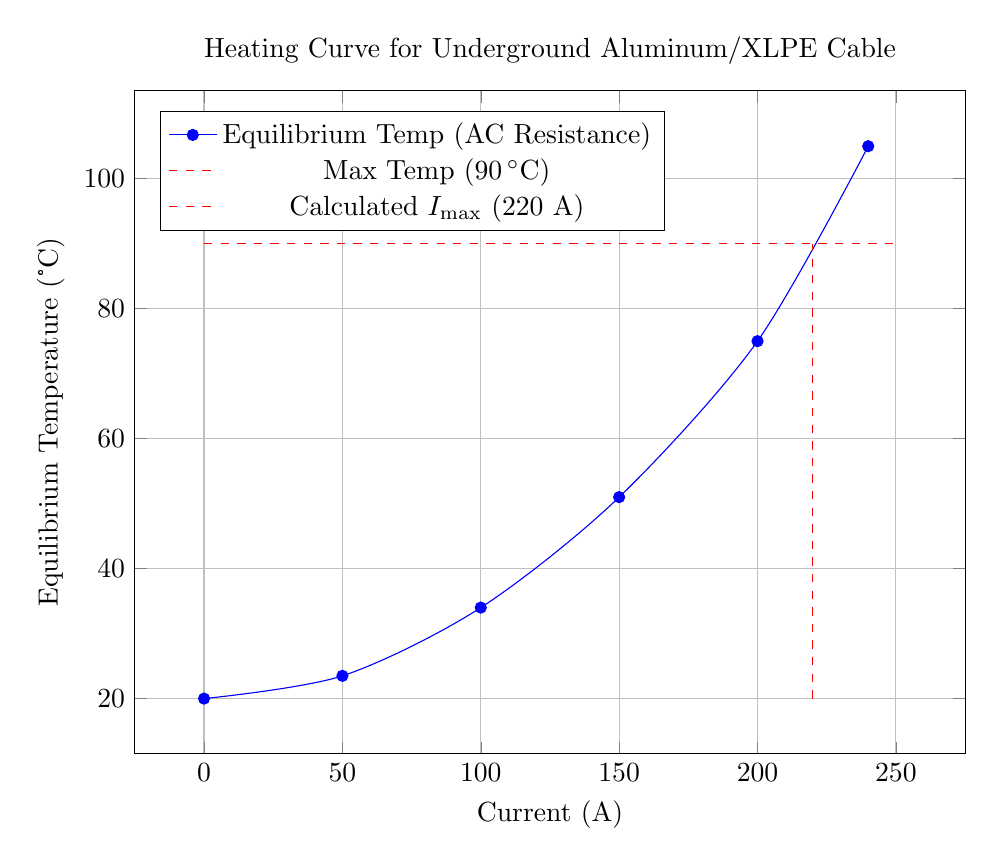
\begin{tikzpicture}
        \begin{axis}[
            title={Heating Curve for Underground Aluminum/XLPE Cable},
            xlabel={Current (A)}, ylabel={Equilibrium Temperature (°C)},
            width=\textwidth, height=10cm, grid=major, legend pos=north west,
        ]
        \addplot[smooth, mark=*, blue] coordinates {(0,20) (50,23.5) (100,34) (150,51) (200,75) (240,105)};
        \addlegendentry{Equilibrium Temp (AC Resistance)}
        
        \addplot[dashed, color=red] coordinates {(0,90) (250,90)};
        \addlegendentry{Max Temp (\SI{90}{\celsius})}

        \addplot[dashed, color=red] coordinates {(220,20) (220,90)};
        \addlegendentry{Calculated $I_{\text{max}}$ (220 A)}
        \end{axis}
    \end{tikzpicture}
    \caption{Equilibrium conductor temperature as a function of load current.}
    \label{fig:heating_curve}
\end{figure}

\begin{figure}[h!]
    \centering
    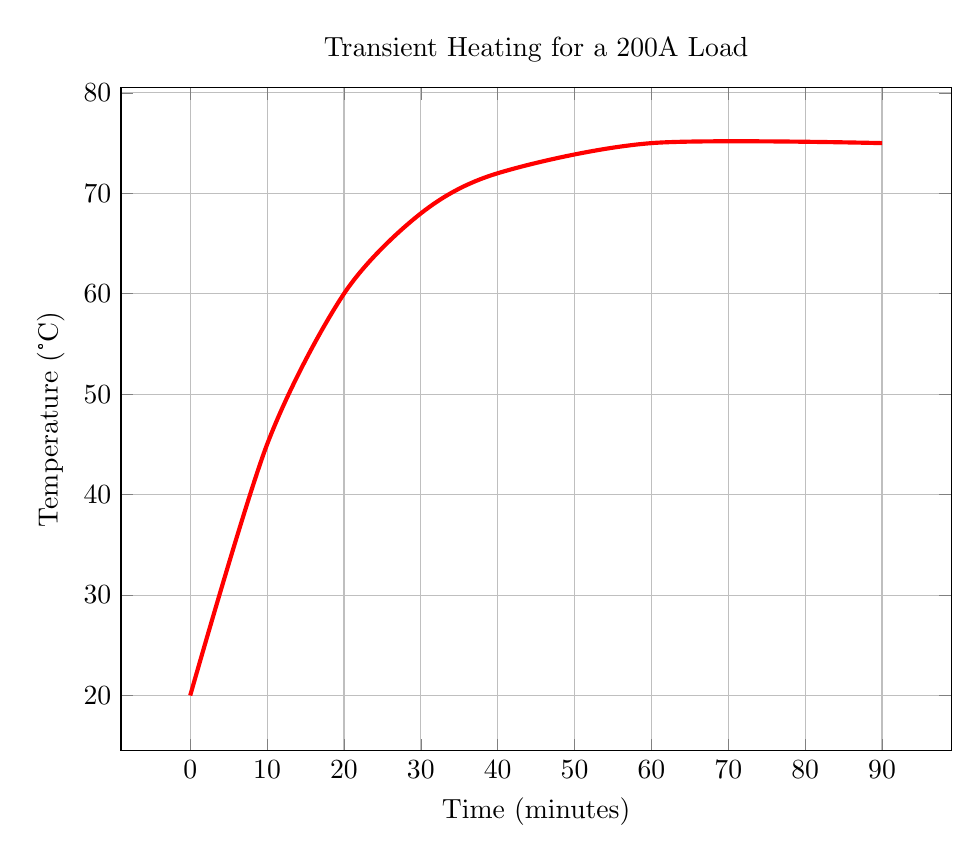
\begin{tikzpicture}
        \begin{axis}[
            title={Transient Heating for a 200A Load},
            xlabel={Time (minutes)}, ylabel={Temperature (°C)},
            width=\textwidth, height=10cm, grid=major,
        ]
        \addplot[smooth, mark=none, red, line width=1.5pt] coordinates {(0,20) (10,45) (20,60) (30,68) (40,72) (60,75) (90,75)};
        \end{axis}
    \end{tikzpicture}
    \caption{Transient temperature response of the conductor over time.}
    \label{fig:transient_heating}
\end{figure}

If we compare both graphs, we see that the steady state temperature reached by the transitive simulation is the same as the temperature shown in the heating curve for the same current.





\newpage
% --- CHAPTER 2: VOLTAGE DROP ANALYSIS ---
\section{Advanced Voltage Drop Analysis}
This section details a precise voltage drop analysis, including reactive effects, based on the MATLAB functions prefixed with 'F'.

\subsection{Blondel's Formula}
The approximate voltage drop in a three-phase AC circuit is calculated using Blondel's formula, which is valid for most well designed circuits where the angle between the voltage at the source and at the load is very small. The script (\texttt{F2\_calculateExactVoltageDrop.m} is used, which accounts for both resistance ($R$) and inductive reactance ($X_L$). Where d is a configuration parameter and takes the value of d = 2 for a single phase line with return and d = 1.732 for three phase lines.
\begin{equation}
    \Delta V = \sqrt{3} \cdot I \cdot (R \cos\varphi + X_L \sin\varphi)
\end{equation}

    
    
    
    
    
    
    
    
    
    
    
    
\subsection{REBT Compliance and Voltage Profile}
Compliance with the Spanish regulation (REBT) is mandatory. The script \texttt{F4b\_checkInstallationCompliance.m} automates checking the tiered voltage drop limits for a full installation (LGA, DI, etc.). The script \texttt{F6\_plotInstallationProfile.m} visualizes this drop, as shown in Figure \ref{fig:installation_profile}.
In the case shown in the graph, the installation does not meet the REBT criteria as it goes beyond the 5\% voltage drop limit. In this case, the installation parameters would have to be revised, most likely by increasing the conductor cross section, in order to further decrease the voltage drop. 

\begin{figure}[h!]
    \centering
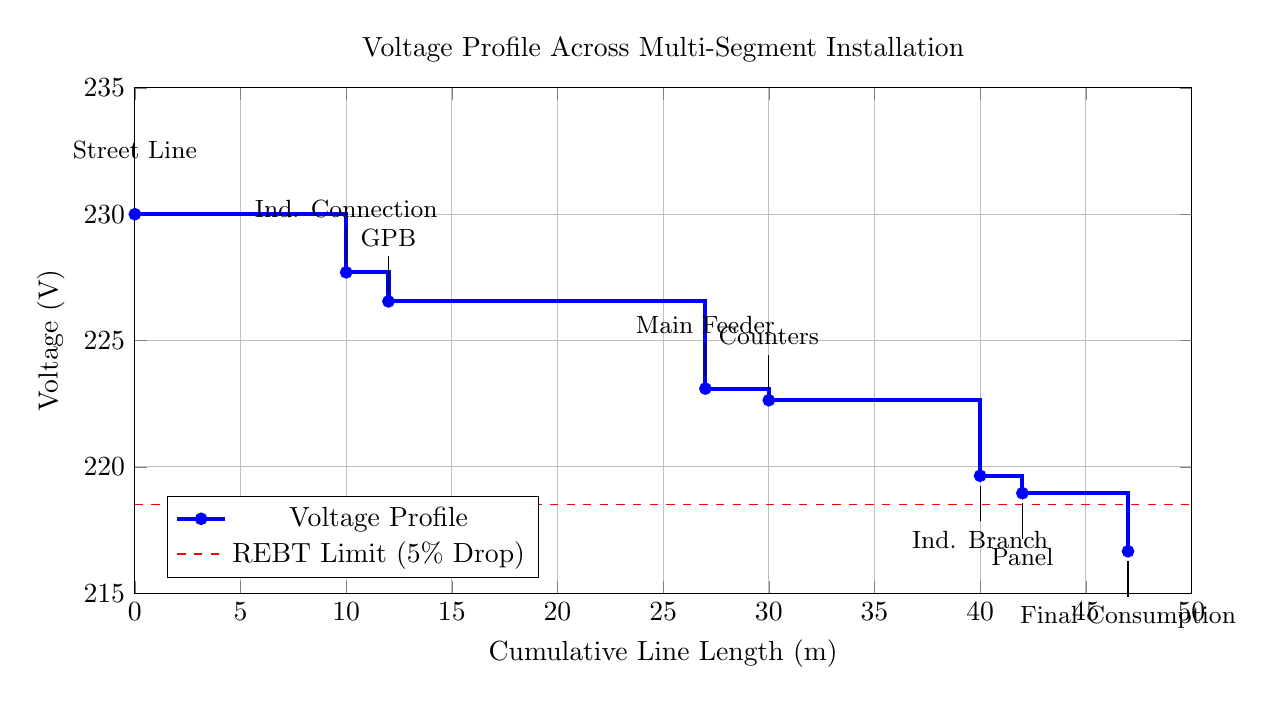
\begin{tikzpicture}
    \begin{axis}[
        title={Voltage Profile Across Multi-Segment Installation},
        xlabel={Cumulative Line Length (m)},
        ylabel={Voltage (V)},
        width=15cm, 
        height=8cm,
        grid=major,
        legend pos=south west,
        xmin=0,
        xmax=50,
        ymin=215,
        ymax=235,
    ]
    
    % The plot with new, detailed coordinates for each stage
    \addplot[const plot, blue, line width=1.5pt, mark=*, mark size=1.5pt] coordinates {
        (0, 230)      % Start
        (10, 227.7)   % Drop 1.0%
        (12, 226.55)  % Drop 0.5%
        (27, 223.1)   % Drop 1.5%
        (30, 222.64)  % Drop 0.2%
        (40, 219.65)  % Drop 1.3%
        (42, 218.96)  % Drop 0.3%
        (47, 216.66)  % Drop 1.0%
    };
    \addlegendentry{Voltage Profile}
    
    % The 5% voltage drop limit line
    \addplot[dashed, color=red] coordinates {(0, 218.5) (50, 218.5)};
    \addlegendentry{REBT Limit (5\% Drop)}

    % Define coordinates for the pin labels
    \coordinate (p0) at (axis cs:0, 230);
    \coordinate (p1) at (axis cs:10, 227.7);
    \coordinate (p2) at (axis cs:12, 226.55);
    \coordinate (p3) at (axis cs:27, 223.1);
    \coordinate (p4) at (axis cs:30, 222.64);
    \coordinate (p5) at (axis cs:40, 219.65);
    \coordinate (p6) at (axis cs:42, 218.96);
    \coordinate (p7) at (axis cs:47, 216.66);
    
    \end{axis}
    
    % Add annotations using pins attached to the coordinates.
    % Placed outside the 'axis' environment to prevent clipping.
    \node[pin={[pin edge={black, thin}, text=black, font=\small]90:{Street Line}}] at (p0) {};
    \node[pin={[pin edge={black, thin}, text=black, font=\small]90:{Ind. Connection}}] at (p1) {};
    \node[pin={[pin edge={black, thin}, text=black, font=\small]90:{GPB}}] at (p2) {};
    \node[pin={[pin edge={black, thin}, text=black, font=\small]90:{Main Feeder}}] at (p3) {};
    \node[pin={[pin edge={black, thin}, text=black, font=\small]90:{Counters}}] at (p4) {};
    \node[pin={[pin edge={black, thin}, text=black, font=\small]-90:{Ind. Branch}}] at (p5) {};
    \node[pin={[pin edge={black, thin}, text=black, font=\small]-90:{Panel}}] at (p6) {};
    \node[pin={[pin edge={black, thin}, text=black, font=\small]-90:{Final Consumption}}] at (p7) {};
    
\end{tikzpicture}
    \caption{Voltage profile across an installation, showing the drop at each section.}
    \newpage
\newpage
    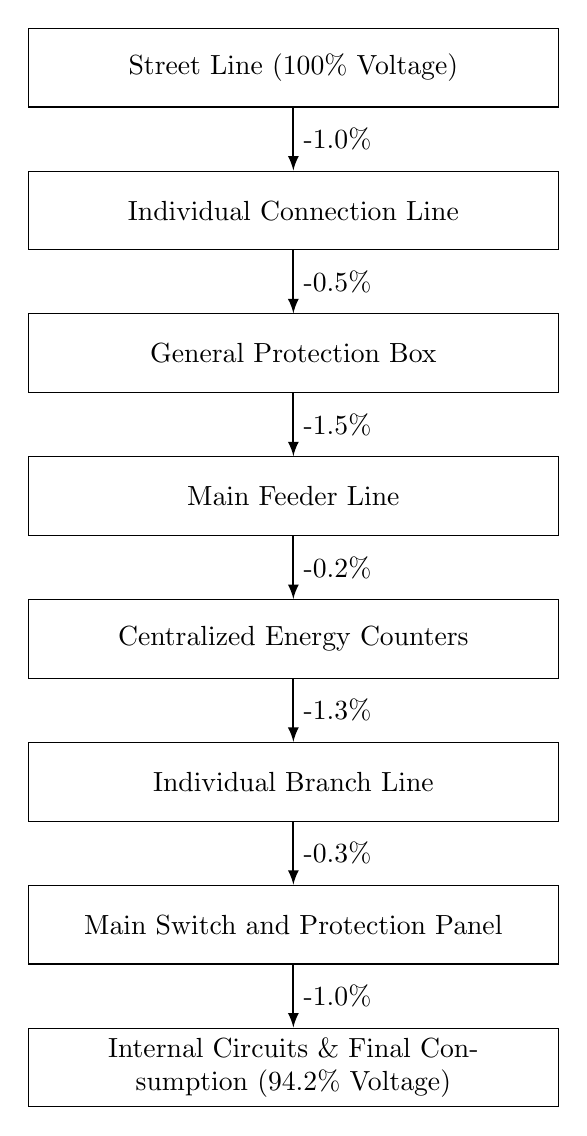
\begin{tikzpicture}[
    node distance=0.8cm, % Vertical distance between boxes
    box/.style={
        draw,
        rectangle,
        text width=6.5cm,
        align=center,
        minimum height=1cm
    },
    arrow/.style={
        -latex,
        thick
    }
]
    % --- Nodes arranged vertically for a clear top-to-bottom flow ---
    \node[box] (start)    {Street Line (100\% Voltage)};
    \node[box, below=of start] (conn)     {Individual Connection Line};
    \node[box, below=of conn]  (gpb)      {General Protection Box};
    \node[box, below=of gpb]   (feeder)   {Main Feeder Line};
    \node[box, below=of feeder] (counters) {Centralized Energy Counters};
    \node[box, below=of counters](branch)  {Individual Branch Line};
    \node[box, below=of branch] (panel)    {Main Switch and Protection Panel};
    \node[box, below=of panel]  (end)      {Internal Circuits \& Final Consumption (94.2\% Voltage)};

    % --- Arrows with simplified labels showing only the drop at each stage ---
    \draw[arrow] (start)    -- node[midway, right] {-1.0\%} (conn);
    \draw[arrow] (conn)     -- node[midway, right] {-0.5\%} (gpb);
    \draw[arrow] (gpb)      -- node[midway, right] {-1.5\%} (feeder);
    \draw[arrow] (feeder)   -- node[midway, right] {-0.2\%} (counters);
    \draw[arrow] (counters) -- node[midway, right] {-1.3\%} (branch);
    \draw[arrow] (branch)   -- node[midway, right] {-0.3\%} (panel);
    \draw[arrow] (panel)    -- node[midway, right] {-1.0\%} (end);
\end{tikzpicture}

    \label{fig:installation_profile}
\end{figure}
    
    \newpage

% --- CHAPTER 3: CONDUCTOR SIZING ---
\section{Conductor Sizing and Economic Analysis}
The final step is to select the optimal conductor cross-section. This analysis, based on the 'G' series of MATLAB scripts, integrates technical requirements with long-term economic factors.

\subsection{Technical and Economic Sizing Criteria}
Conductor sizing is based on two main criteria:
\begin{enumerate}
    \item \textbf{Technical Minimum:} The smallest standard cross-section that satisfies both the maximum admissible current ($I_{\text{max}}$) and the REBT voltage drop limits. This is calculated via \texttt{G2\_calculateRequiredSection.m} and \texttt{G3\_selectStandardSection.m}.
    \item \textbf{Economic Optimum:} The cross-section that results in the lowest total lifecycle cost (LCC), considering both the initial cable purchase price and the cumulative cost of energy losses ($I^2R$) over the project's lifespan. This is a simpler, albeit similar approach to Kelvin's Economic Law for calculating the economic conductor size.
    
    \begin{figure}[h!]
    \centering
    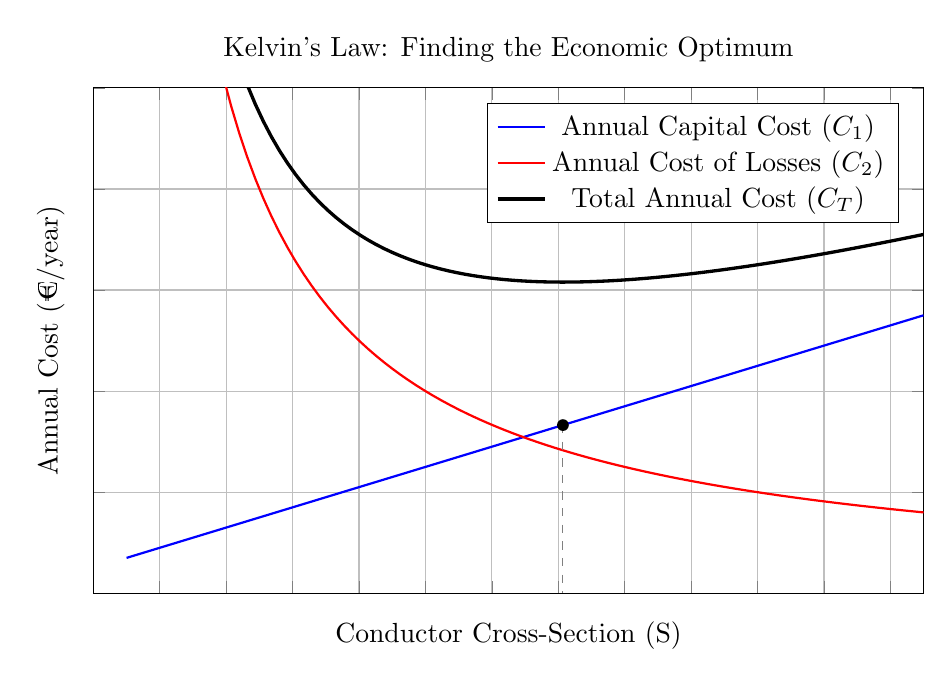
\begin{tikzpicture}
        \begin{axis}[
            title={Kelvin's Law: Finding the Economic Optimum},
            xlabel={Conductor Cross-Section (S)},
            ylabel={Annual Cost (€/year)},
            width=\textwidth,
            height=8cm,
            grid=major,
            legend pos=north east,
            xmin=0, xmax=250,
            ymin=0, ymax=100,
            xticklabel=\empty, yticklabel=\empty,
        ]
        
        % C1: Capital Cost (approximated as linear for simplicity in the graph)
        \addplot[domain=10:250, blue, thick, samples=100] {0.2*x + 5};
        \addlegendentry{Annual Capital Cost ($C_1$)}

        % C2: Cost of Losses (inversely proportional)
        \addplot[domain=10:250, red, thick, samples=100] {4000/x};
        \addlegendentry{Annual Cost of Losses ($C_2$)}
        
        % CT: Total Cost (sum of the two)
        \addplot[domain=10:250, black, very thick, samples=100] {0.2*x + 5 + 4000/x};
        \addlegendentry{Total Annual Cost ($C_T$)}

        % Mark the optimal point
        \coordinate (opt) at (axis cs:141.4, 33.28);
        \draw[dashed, gray] (opt) -- (opt |- {axis cs:0,0});
        \node[below] at (opt |- {axis cs:0,0}) {$S_{\text{opt}}$};
        \node[circle, fill, inner sep=1.5pt] at (opt) {};
        
        \end{axis}
    \end{tikzpicture}
    \caption{The optimal conductor size ($S_{\text{opt}}$) occurs at the minimum of the total annual cost curve, which corresponds to the point where the cost of losses and the annualized capital cost curves intersect.}
\end{figure}
\end{enumerate}

\subsection{Lifecycle Cost Analysis}
The lifecycle cost is modeled in \texttt{G4\_calculateLifecycleCost.m} as:
\begin{equation}
    C_{\text{total}} = C_{\text{initial\_cable}} + C_{\text{energy\_losses}}
\end{equation}
While a smaller cable is cheaper initially, it has higher resistance and thus a higher cost of energy losses over time. A larger, more expensive cable has lower losses. The optimal size minimizes this sum.

\subsection{Sizing Analysis Results}
The economic analysis is visualized in Figure \ref{fig:economic_analysis}. The stacked bars show the components of the total cost, while the red line shows the total LCC. The analysis identifies both the smallest technically compliant section and the larger, economically optimal section, which provides long-term savings.

\begin{figure}[h!]
    \centering
    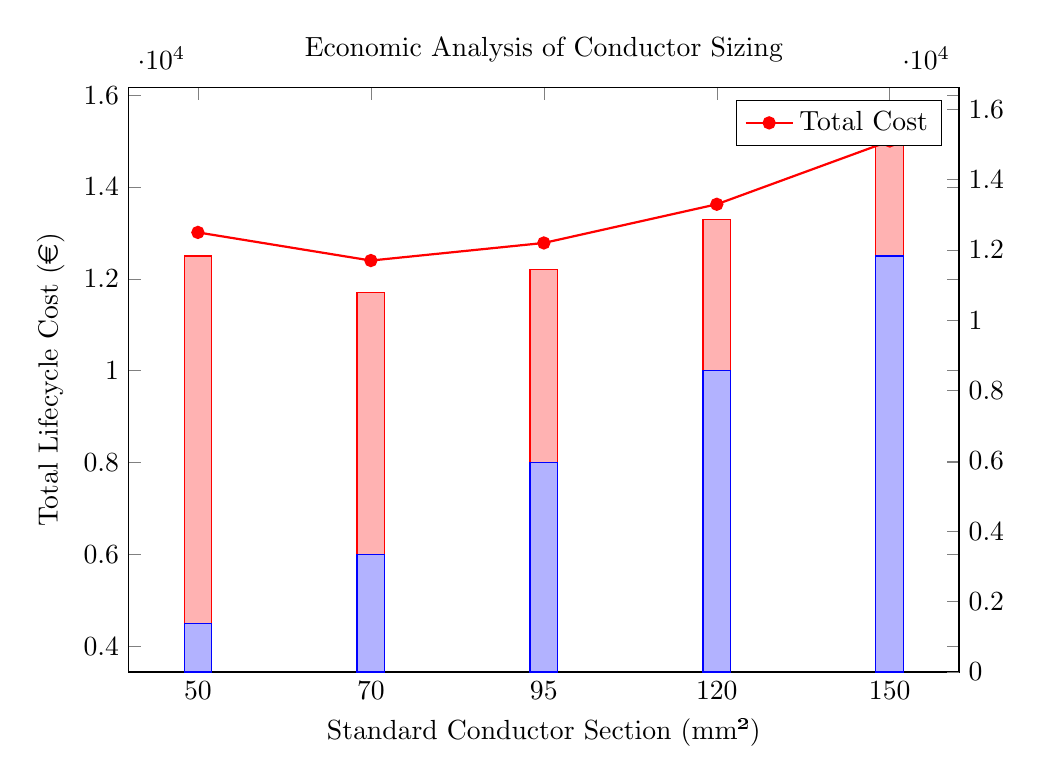
\begin{tikzpicture}
        \begin{axis}[
            ybar stacked,
            title={Economic Analysis of Conductor Sizing},
            xlabel={Standard Conductor Section (mm²)},
            ylabel={Total Lifecycle Cost (\euro{})},
            width=\textwidth, height=9cm,
            symbolic x coords={50, 70, 95, 120, 150},
            xtick=data,
            legend style={at={(0.5,-0.2)}, anchor=north, legend columns=-1},
        ]
        \addplot coordinates {(50, 4500) (70, 6000) (95, 8000) (120, 10000) (150, 12500)}; % Total Lif Cost
        \addplot coordinates {(50, 8000) (70, 5700) (95, 4200) (120, 3300) (150, 2600)}; % Loss Cost
        \end{axis}
        
        \begin{axis}[
            width=\textwidth, height=9cm, axis y line*=right, axis x line=none,
            ylabel near ticks,
            symbolic x coords={50, 70, 95, 120, 150},
            xtick=data,
            ymin=0,
        ]
        \addplot[red, thick, mark=*, mark options={fill=red}] coordinates {(50, 12500) (70, 11700) (95, 12200) (120, 13300) (150, 15100)};
        
        \legend{Total Cost, Energy Loss Cost, Total LCC}
        
        \end{axis}
    \end{tikzpicture}
    \caption{Lifecycle cost analysis identifying the technically minimum (50 mm²) and economically optimal (70 mm²) sections.}
    \label{fig:economic_analysis}
\end{figure}

% --- CONCLUSION ---
\section{Conclusion}
The Week 2 analysis has significantly advanced the project by incorporating critical thermal, reactive, and economic effects into the line design process. The modular MATLAB toolkit provides a powerful framework for accurately dimensioning conductors based on a detailed understanding of their performance under real-world loads. This framework is completed with the conductor sizing module, which integrates technical constraints (voltage drop and ampacity) with economic analysis (lifecycle cost) to determine the optimal conductor cross-section, providing a comprehensive solution that balances performance, safety, and cost.






\end{document}